% \documentclass[12pt, twoside]{article}
\usepackage[letterpaper, margin=1in, headsep=0.2in]{geometry}
\setlength{\headheight}{0.6in}
%\usepackage[english]{babel}
\usepackage[utf8]{inputenc}
\usepackage{microtype}
\usepackage{amsmath}
\usepackage{amssymb}
%\usepackage{amsfonts}
\usepackage[nomessages]{fp} %\FPeval{\var-name}{2*sin(pi/6)}
\usepackage{siunitx} %units in math. eg 20\milli\meter
\usepackage{yhmath} % for arcs, overparenth command
\usepackage{tikz} %graphics
\usetikzlibrary{quotes, angles, arrows, arrows.meta}
\usepackage{graphicx} %consider setting \graphicspath{{images/}}
\usepackage{parskip} %no paragraph indent
\usepackage{enumitem}
\usepackage{multicol}
\usepackage{venndiagram}

\usepackage{fancyhdr}
\pagestyle{fancy}
\fancyhf{}
\renewcommand{\headrulewidth}{0pt} % disable the underline of the header
\raggedbottom
\hfuzz=2mm %suppresses overfull box warnings

\usepackage{hyperref}

\fancyhead[LE]{\thepage}
\fancyhead[RO]{\thepage \\ Name: \hspace{4cm} \,\\}
\fancyhead[LO]{BECA / Dr. Huson / Geometry\\*  Unit 8: Regents review\\* 2 March 2023}

\begin{document}

\subsubsection*{8.5 Classwork: Analytic geometry \hfill 8.F.A.3}
\begin{enumerate}

\item A line is plotted in the graph below.
\begin{multicols}{2}
    \begin{enumerate}[itemsep=0.5cm]
      \item Write down the $y$-intercept of the line.
      \item What is the slope of the line?
      \item What is the $x$-intercept of the line?
      \item Write down its equation in slope-intercept form.
      \end{enumerate}
    \begin{flushright}
    \begin{tikzpicture}[scale=0.8]
      \draw [help lines] (-1,-2) grid (6,5);
      \draw [thick, ->] (-1.2,0) -- (6.6,0) node [above right] {$x$};
      \draw [thick, ->] (0,-2.2)--(0,5.4) node [right] {$y$};
      \draw [fill] (0,3) circle [radius=0.05] node[above right] {$(0,3)$};
      \draw [fill] (6,0) circle [radius=0.05] node[below left] {$(6,0)$};
      \draw [<->, thick, domain=-0.5:6.8] plot (\x,-0.5*\x+3);
    \end{tikzpicture}
    \end{flushright}
  \end{multicols} \vspace{2cm}

\item Find the slope of the line through the points $(-1, 4)$ and $(1, 6)$. \vspace{3cm}

\item A line has a slope of $\displaystyle \frac{3}{5}$ and passes through the point $(10, 7)$. 
  \begin{enumerate}[itemsep=1cm]
      \item Write the equation of the line in the form $(y-y_1)=m(x-x_1)$.
      \item Rewrite the equation of the line in the form $y=mx+b$. \vspace{4cm}
  \end{enumerate}

\newpage
\subsubsection*{Systems of equations \hfill HSG.REI.C.6}
\item Dr. Huson buys six pizza pies for the Pi Day party, some plain, some special with all the toppings. Plain pizzas cost \$10 and ``everything'' pizzas \$15. The total cost was \$70. How many of each pizza did he buy?
\begin{flushright}
  \begin{tikzpicture}[scale=.65]
    \draw [help lines] (0,0) grid (12,12);
    \draw [thick, ->] (0,0) -- (12.4,0) node [above right] {$x$};
    \draw [thick, ->] (0,0)--(0,12.4) node [right] {$y$};
    \foreach \x in {1,...,12}
    \draw[shift={(\x,0)}] (0pt,-3pt)--(0pt,3pt) node[below=5pt] {$\x$};
    \foreach \y in {1,...,12}
    \draw[shift={(0,\y)}] (-3pt,0pt)--(3pt,0pt) node[left=5pt] {$\y$};
  \end{tikzpicture}
  \end{flushright}

\item Graph and label the two equations. Mark their intersection as an ordered pair.
  \begin{multicols}{2}
    $f(x) = -x+5$ \\
    $g(x) = \frac{3}{4}x-2$
  \end{multicols}
  \begin{center}
  \begin{tikzpicture}[scale=.635]
    \draw [help lines] (-8,-6) grid (10,8);
    \draw [thick, ->] (-8.2,0) -- (10.4,0) node [below right] {$x$};
    \draw [thick, ->] (0,-6.2)--(0,8.4) node [left] {$y$};
  \end{tikzpicture}
  \end{center}

\end{enumerate}
\end{document}